\documentclass[11pt, a4paper]{article}
\usepackage[a4paper, top=20mm, left=18mm, right=18mm, bottom=20mm]{geometry}
\usepackage{hyperref}
\usepackage[sf]{titlesec}
\usepackage{listings}
\usepackage{graphicx}
\usepackage{float}
\usepackage{caption}
\captionsetup{font={sf}}
\usepackage{color}
\hypersetup{hidelinks = true}
\definecolor{codegrey}{rgb}{0.95, 0.95, 0.96}
\lstset{backgroundcolor = \color{codegrey}, basicstyle=\normalsize\ttfamily}
\begin{document}
{\fontfamily{cmss}\selectfont

\title{\vspace{-20mm}CMPUT 291 - Mini Project 2 Design Document}
\date{}
\maketitle
\vspace{-20mm}

\section{Overview and User Guide}\label{OV}
The following software package is comprised of 3 phases. Phase 1 takes email data from an XML file and outputs the data into four files: terms.txt, emails.txt, dates.txt, and recs.txt. Phase 2 sorts these files and builds four indexes. Phase 3 is responsible for data retrieval, and queries the data.

\begin{figure}[H]
\centering
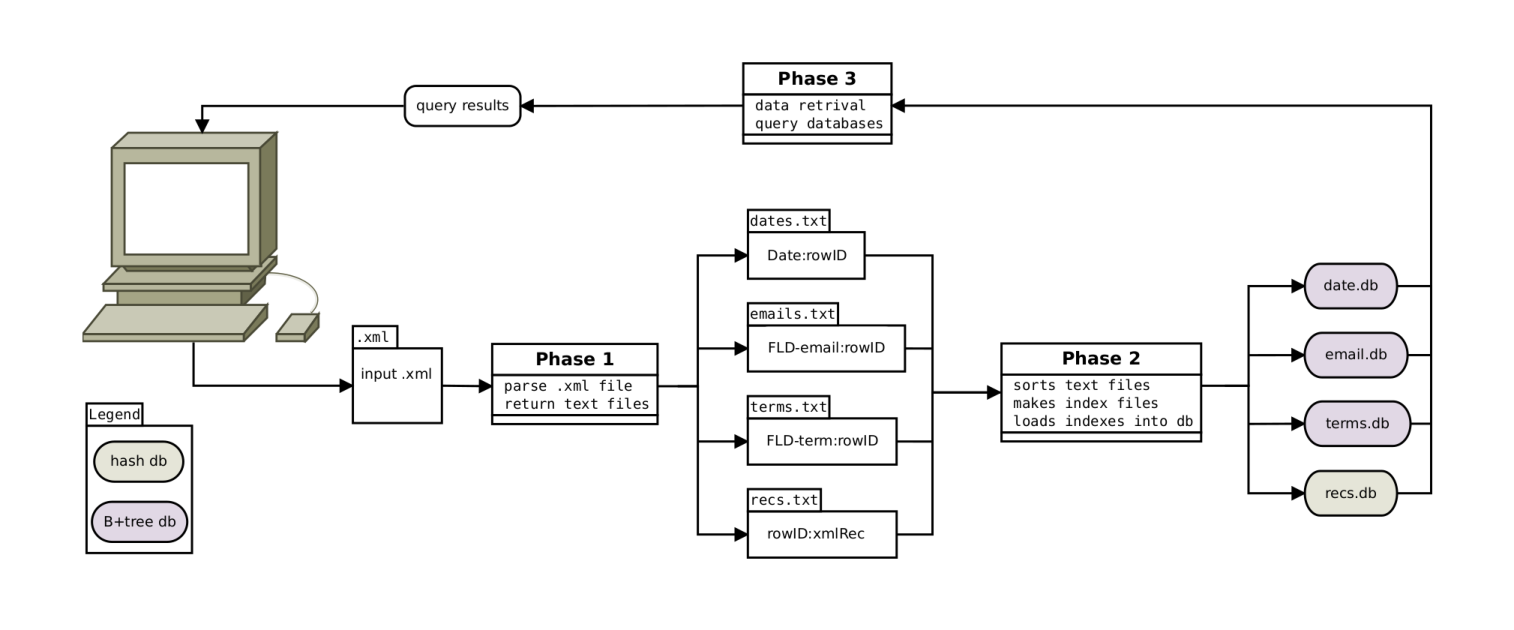
\includegraphics[width = \textwidth]{software_FD.pdf}\label{fig}
\caption{Flow diagram of files, data, and different phases of the software. For more implementation details see \emph{\nameref{SD}}.}
\end{figure}

\subsection{Phase 1: Preparing Data Files}
Preparation of the data files is completed by the python program \texttt{phase1.py}. The software reads in an \texttt{.xml} file specified by the user line by line, parses the line, and writes the data into four output files: \texttt{terms.txt}, \texttt{emails.txt}, \texttt{dates.txt}, and \texttt{recs.txt}. The phase 1 software can be run by entering the following command in the Linux terminal:
\begin{lstlisting}
    $ python3 phase1.py
\end{lstlisting}
The program will prompt the user to enter an \texttt{.xml} file:
\begin{lstlisting}
    Enter .xml file: datafile.xml
\end{lstlisting}
If the provided file is not found, or an incorrect file extension is given, an error message will display, and the user can re-enter a filename. If no extension is specified, the program will assume it is \texttt{.xml}. If the output files already exist in the directory, the program will overwrite the data currently on the files.

\subsection{Phase 2: Building Indexes}
Phase 2 takes the output files from phase 1 and sorts them, and produces four index files from the sorted data: \texttt{te.idx}, \texttt{em.idx}, \texttt{da.idx}, \texttt{re.idx}. If the index files already exist from a previous run, the data on them will be overwritten.

The index files are then loaded into four databases: \texttt{terms.db}, \texttt{email.db}, \texttt{date.db}, \texttt{recs.db}. Once again, if these databases are already found in the directory, they will be overwritten by the new data. 

No user input is required for phase 2. To build the indexes, simply execute the following command in the terminal:
\begin{lstlisting}
    $ python3 phase2.py
\end{lstlisting}
\subsection{Phase 3: Data Retrieval}
Phase 3 provides the user a simple interface to query the data prepared in phases 1 and 2. The query program uses \emph{Berkeley DB} to process the queries entered by the user. The user can query dates, emails, or terms. Depending on the type of query, it will have different formats. In general, queries are of the form:
\begin{lstlisting}
    > prefix:query
\end{lstlisting}

A date query will return all emails with dates that satisfy the query.
\begin{lstlisting}
    > date(:|>|<|>=|<=)YYYY/MM/DD
\end{lstlisting}

An email query returns all emails sent to/from/cc/bcc the email address specified:
\begin{lstlisting}
    > (to|from|cc|bcc):email@address.com
\end{lstlisting}

A term query returns all records that have the term in their subject or body field (field specified by user)
\begin{lstlisting}
    > (subj|body):term
\end{lstlisting}

Terms can also be queried without specifying the field. For example,
\begin{lstlisting}
    > confidential%
\end{lstlisting}
will return all records that have a term with prefix \emph{confidential} in their subject or body fields (confidential, confidentially, confidentiality, etc.).
 
The program will ignore all white spaces in the entered queries, so
\begin{lstlisting}
    > subj :   gas        body:earning
\end{lstlisting}
will successfully search the data for records that have gas in their subject and earning in their body fields. All queries are case-insensitive as well.

\section{Query Algorithms}\label{SD}
The query algorithm used in this program operates by first evaluates each query the user enters individually,then takes the intersection of all queries to generate a master list of row IDs. Each ID in the master list is used to complete an equality search on the records database to generate the results that match all of the queries.\newline

\noindent This algorithm is effficient in that it eliminates redundancy, while retaining accuracy. Since each query is completed at least once we can quarantee no results are missed, and since each query is completed at most once (including the query of the records database with the rowIDs), we are reducing the amount of redundant searches. One caveat of this system is that it does check to see if a key was already searched for (for example, if an equality search was already completed in a previous range search). This feature could be implemented at the cost of space.\newline

\noindent A seperate strategy is used to calculate each query depending on if the query requires an equality or range search of the items in the database, and if the query is a term query containing the wild card \emph{(\%)} operator or not.

\begin{itemize}

\item Equality Search
	\begin{quotation}
	\noindent The program executes equality searches by setting the cursor of the database to the provided key (term, date or email term), then adding all items to a set (to prevent redundancy) that have the same key (iterated by using the \emph{cursor.next\_dup()} command). The resulting set is returned.
	\end{quotation}	

\item Range Search
	\begin{quotation}
	\noindent There are two types of range search: a greater-than search and a less-than search. Both utilize a similar stratgey but the program distinguishes between both for simplicity:
	\begin{itemize}
		\item Greater-Than Search
		\begin{quotation}
		\noindent The greater-than search first moves the cursor to the specified key (or the value directly after the key if it is not inclusive), then moves the database cursor along the rest of the database. Each item is added to a set of RowIDs as the database is traversed.
		\end{quotation}
		\item Less-Than Search
		\begin{quotation}
		\noindent The less-than search first moves the cursor to the first key in the database, then moves the database cursor along the database until the cursor reaches the key. Each item is added to a set of RowIDs as the database is traversed. If the search is exclusive, the query does not add the items corresponing to the provided key.
		\end{quotation}
	\end{itemize}
	\end{quotation}

\item Wild Card
	\begin{quotation}
	\noindent Wild card searches are handled similarily to range searches in that the database is traversed along a set of key-value pairs, with each value being added to a set. To do this the program moves the cursor to the specified key (without the wild card) and traverses the database until it reaches a key that does not have the provided key as a prefix. 
	\end{quotation}	
\end{itemize}


\section{Testing Strategy}\label{TS}
All functions were tested extensively throughout development, and again after completion of the program. Both the brief and full output modes were tested, as well as those cases in which no results exist. Specific general test cases are listed below.
\begin{itemize}

\item Individual \& Multiple Term Queries (combination of subj:term, body:term, term and term\% on same line)
\item Individual \& Multiple Date Queries (combination of date:key, date<key, date<=key, date>key and date>=key on same line)
\item Individual \& Multiple Email Queries (combination of to:key, from:key, cc:key and bcc:key on same line)
\item Individual \& Multiple Combination of Queries (combination of different term, email and date queries on same line)

\end{itemize}
 

\section{Group Work}\label{GW}
\begin{itemize}

\item Phase 1: Dalton: 
	
\item Phase 2: Harrison \& Dalton: Collaborative, 1hrs
	
\item Phase 3: Get Queries, Display Results (Brief and Full Output), Query Records, Get Field Functions, Parsing Queries
	\begin{itemize}
	\item Dalton: 
	\end{itemize}
	
\item Phase 3: Email, Term and Date Queries, Equality and Range Search Functions:
	\begin{itemize}
	\item Harrison: 3 hrs
	\end{itemize}
	
\item Design Document
	\begin{itemize}
	\item Dalton:
	\item Harrison: 1 hrs
	\end{itemize}
	
\item Testing and Code Quality
	\begin{itemize}
	\item Dalton:
	\item Harrison: 1.5 hrs
	\end{itemize}

\end{itemize}


\end{document}
